\chapter{Pendahuluan}
\label{chap:intro}

Bab ini menjelaskan tentang latar belakang yang menjadi dasar pengerjaan dari penelitian pada tugas akhir ini. Kemudian, dijelaskan mengenai rumusan masalah, tujuan, serta batasan masalah yang membahas ruang lingkup dari penelitian ini. Kemudian, dibahas juga mengenai metodologi penelitian yang menjelaskan mengenai langkah-langkah penyelesaian berdasarkan rumusan masalah yang sudah didefinisikan. Bagian ini diakhiri dengan sistematika pembahasan yang menguraikan isi dari setiap bab pada laporan tugas akhir ini.

\section{Latar Belakang}
\label{sec:1:latar_belakang}

\begin{figure}[h]
\centering
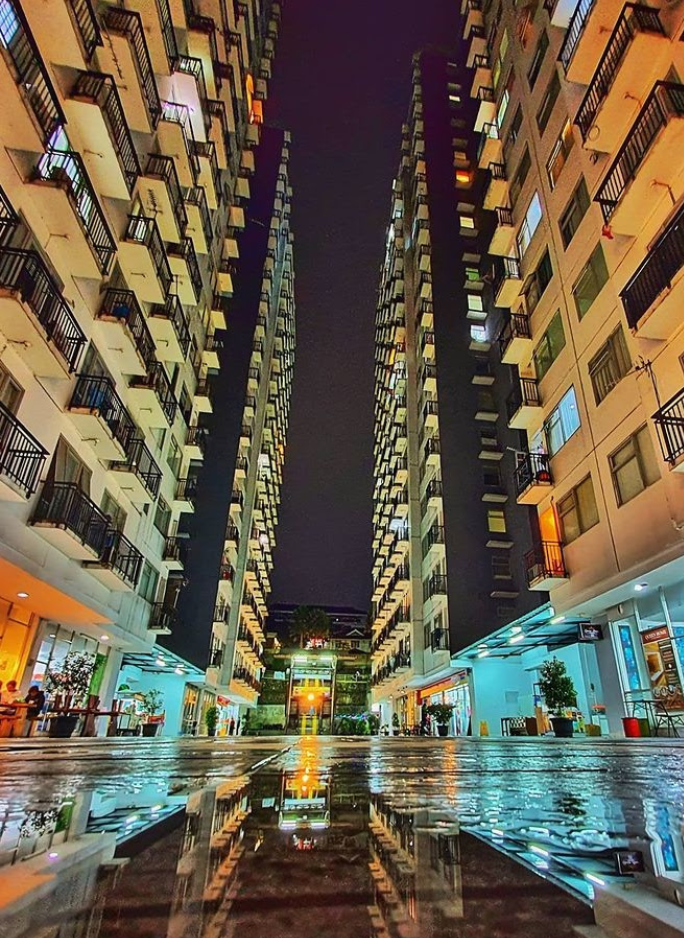
\includegraphics[width=0.45\textwidth]{Gambar/The-Jarrdin-Beranda-crop.png}
\caption{Rusunami The Jarrdin Cihampelas}
\label{fig:the jardin}
\end{figure}

Rusunami The Jarrdin Cihampelas (RTJC) merupakan kompleks hunian vertikal yang terletak di kawasan strategis Cihampelas, Kota Bandung. RTJC terdiri dari empat {tower} dengan lebih dari 2.400 unit hunian, dilengkapi dengan area komersial, kolam renang, dan fasilitas parkir bertingkat\footnote{\url{https://thejarrdin.com/}, diakses pada 17 Maret 2025}. Letaknya yang berdekatan dengan destinasi wisata populer seperti Teras Cihampelas dan Cihampelas Walk menjadikan hunian ini memiliki tingkat okupansi yang tinggi, baik oleh wisatawan, mahasiswa, maupun pekerja dari luar kota, dengan durasi sewa yang bervariasi dari jangka pendek hingga jangka panjang.

Sistem penyewaan di RTJC dijalankan melalui dua jalur utama, yaitu secara langsung oleh pemilik unit atau melalui perantara agen properti. Secara operasional, pengelolaan lingkungan hunian beserta aktivitas penyewaan ini dikoordinasikan oleh \textbf{Paguyuban Komersial Jarrdin (PKJ)}, \textbf{Perhimpunan Pemilik dan Penghuni Satuan Rumah Susun (P3SRS)}, serta \textbf{ketua agen}—yang selanjutnya disebut sebagai \textbf{Pengelola}. Pihak Pengelola ini bertanggung jawab penuh atas tata kelola, penerimaan titipan penyewaan, serta menjaga ketertiban umum. Meskipun tingginya mobilitas penyewa memberikan keuntungan ekonomi, namun hal ini juga menghadirkan tantangan signifikan bagi Pengelola dalam aspek pengawasan dan keamanan.

Tantangan nyata yang dihadapi adalah munculnya aktivitas ilegal di lingkungan hunian. Sepanjang tahun 2024, tercatat setidaknya 15 kasus pelanggaran hukum di lingkungan RTJC, meliputi praktik prostitusi terselubung, penyalahgunaan narkoba, serta tindak kriminal lainnya. Kasus-kasus ini umumnya terungkap melalui laporan warga, patroli keamanan rutin, atau saat dilakukan pelayanan kebersihan. Meskipun pihak Pengelola telah menerapkan prosedur preventif seperti penjagaan fisik dan verifikasi identitas penyewa, pendekatan yang masih bersifat {manual} terbukti belum cukup efektif dan responsif dalam mengidentifikasi penyewa yang memiliki potensi pelanggaran. Permasalahan ini mengindikasikan urgensi akan adanya sistem deteksi dini yang mampu mengenali pola perilaku penyewa mencurigakan berdasarkan data historis. 

% Ketersediaan data penyewa yang telah diberi label (normal dan tidak normal) memungkinkan penerapan teknologi \textit{machine learning}, khususnya pendekatan \textit{supervised learning}, untuk membangun model klasifikasi.

% \textit{Supervised learning} melatih model menggunakan data berlabel untuk mempelajari pola perilaku dan menghasilkan prediksi klasifikasi terhadap data penyewa baru. Beberapa algoritma yang potensial untuk diterapkan dalam kasus ini meliputi \textit{Decision Tree, Random Forest, Support Vector Machine} (SVM), {\it K-Nearest Neighbors} (KNN), dan \textit{XGBoost}.

% Selain pengembangan model klasifikasi, diperlukan pula sebuah platform untuk input data dan distribusi hasil analisis. Oleh karena itu, penelitian ini juga mencakup pengembangan sistem berbasis web menggunakan teknologi \textbf{Node.js}. Pemilihan \textbf{Node.js} didasarkan pada pertimbangan interoperabilitas dan kemudahan integrasi dengan ekosistem sistem lain yang dikembangkan oleh rekan mahasiswa di bawah bimbingan dosen yang sama, sehingga menjamin kompatibilitas antar-modul. Di sisi lain, bahasa pemrograman \textbf{Python} digunakan secara khusus untuk tahap pembangunan dan pelatihan model \textit{machine learning} mengingat kelengkapan pustaka \textit{data science} yang dimilikinya. Sistem terintegrasi ini dirancang untuk mempermudah para agen dalam melakukan input data penyewa dan menerima notifikasi hasil klasifikasi secara \textit{real-time} bila terdeteksi adanya penyewa yang berpotensi melakukan pelanggaran. Integrasi antara model klasifikasi berbasis Python dan sistem aplikasi web berbasis Node.js ini diharapkan dapat memberikan kontribusi nyata dalam meningkatkan keamanan hunian vertikal RTJC secara proaktif, efisien, dan berbasis data.

\section{Rumusan Masalah}
\label{sec:rumusan}
Berdasarkan latar belakang dan identifikasi permasalahan yang telah dijelaskan, maka rumusan masalah dalam penelitian ini adalah sebagai berikut.
\begin{enumerate}
    \item Bagaimana pola perilaku penyewa di RTJC dan langkah-langkah antisipatif apa yang telah diterapkan dalam mencegah aktivitas ilegal?
    \item Model klasifikasi apa yang paling sesuai untuk mendeteksi perilaku penyewa mencurigakan di RTJC?
    \item Bagaimana membangun model klasifikasi yang paling sesuai untuk mendeteksi perilaku penyewa mencurigakan di RTJC?
    \item Bagaimana membangun sistem berbasis Node.js yang dapat mengotomatiskan proses identifikasi penyewa mencurigakan dan memberikan informasi kepada pemangku kepentingan?
\end{enumerate}

\section{Tujuan}
\label{sec:tujuan}
Mengacu pada rumusan masalah di atas, tujuan dari penelitian ini adalah sebagai berikut.
\begin{enumerate}
    \item Menganalisis pola perilaku penyewa di RTJC dan mengetahui langkah-langkah antisipatif yang telah diterapkan dalam mencegah aktivitas ilegal.
    \item Menentukan model klasifikasi yang paling sesuai untuk mendeteksi perilaku penyewa mencurigakan di RTJC.
    \item Membangun model klasifikasi yang paling sesuai untuk mendeteksi perilaku penyewa mencurigakan di RTJC.
    \item Membangun sistem berbasis Node.js yang dapat mengotomatiskan proses identifikasi penyewa mencurigakan dan memberikan informasi kepada pemangku kepentingan.
\end{enumerate}


\newpage
\section{Batasan Masalah}
\label{sec:batasan}

Penelitian ini berfokus pada bidang \textit{data science} yang menitikberatkan pada analisis pola perilaku penyewa serta pengembangan perangkat lunak pendukung. Maka ditetapkan batasan-batasan masalah sebagai berikut.

\begin{enumerate}
    \item Data yang digunakan merupakan data historis transaksi penyewaan dan catatan pelanggaran di Rusunami The Jarrdin Cihampelas (RTJC) yang dihimpun dari sebanyak 4 Pelaku Komersil atas dasar kesediaan agen tersebut.
    
    \item Algoritma \textit{machine learning} yang dianalisis dan dibandingkan kinerjanya terbatas pada metode \textit{Supervised Learning}, yaitu \textit{Decision Tree, Random Forest, Support Vector Machine} (SVM), \textit{K-Nearest Neighbors} (KNN), dan \textit{XGBoost}. Klasifikasi yang dilakukan bersifat biner, yaitu mengelompokkan penyewa ke dalam kelas ``normal'' atau ``tidak normal'' (berpotensi melanggar).
    
    \item Sistem aplikasi yang dibangun berfokus pada aspek fungsional utama, yaitu sebagai antarmuka input data bagi agen dan notifikasi hasil deteksi. Pengembangan sistem menggunakan teknologi {Node.js} untuk sisi server dan integrasi sistem, serta {Python} khusus untuk pemrosesan model \textit{machine learning}.
    
    \item Penelitian ini merupakan studi kasus yang spesifik dilakukan di lingkungan Rusunami The Jarrdin Cihampelas (RTJC) bekerja sama dengan Pengelola. Karakteristik data dan pola perilaku yang dihasilkan tidak digeneralisasi untuk seluruh apartemen atau rumah susun di lokasi lain.
    
    \item Aspek non-fungsional sistem seperti keamanan jaringan tingkat lanjut, uji performansi beban server tinggi (\textit{stress testing}), dan penyediaan infrastruktur perangkat keras fisik tidak menjadi fokus utama dalam penelitian ini.

    \item Sebagai bentuk kepatuhan terhadap Undang-Undang Perlindungan Data Pribadi (UU PDP), informasi sensitif penyewa yang mencakup Nomor Induk Kependudukan (NIK) dan nama disamarkan sebagian (\textit{data masking}) pada setiap tampilan antarmuka sistem.
\end{enumerate}



\section{Metodologi}
\label{sec:metlit}
Metodologi penelitian yang digunakan dalam tugas akhir ini dirancang untuk mengembangkan, melatih, serta menguji model klasifikasi perilaku penyewa mencurigakan, sekaligus membangun sistem berbasis Node.js yang dapat mengotomatiskan proses deteksi. Tahapan metodologi penelitian yang dilakukan adalah sebagai berikut.

\begin{enumerate}
    \item \textbf{{Melakukan studi pustaka}} \\
    Studi pustaka dilakukan untuk memahami konsep dasar hunian vertikal dan pola penyewaan di Rusunami The Jarrdin Cihampelas, perilaku penyewa berisiko, serta pendekatan yang digunakan oleh para pengurus di RTJC terkait deteksi aktivitas ilegal. Studi pustaka juga mencakup teori \textit{machine learning}, deteksi anomali (\textit{anomaly detection}), serta model klasifikasi seperti \textit{Decision Tree}, \textit{Random Forest}, \textit{Support Vector Machine} ({SVM}), \textit{K-Nearest Neighbors} ({K-NN}), dan \textit{XGBoost}. Selain itu, dibahas mengenai penanganan ketidakseimbangan kelas melalui \textit{cost-sensitive learning}, konsep \textit{hyperparameter tuning}, teknik \textit{feature engineering}, \textit{feature selection}, evaluasi model dengan metrik presisi dan \textit{recall}, serta literatur mengenai pengembangan sistem berbasis Node.js dan Express.js. Pengenalan teknologi pendukung seperti \textbf{Python}, \textit{Streamlit}, dan Google Cloud Platform (GCP) juga menjadi bagian dari studi pustaka ini.
    
    \item \textbf{{Melakukan survei dan wawancara}} \\
    Tahap ini dilakukan dengan melakukan survei langsung ke lokasi Rusunami The Jarrdin Cihampelas (RTJC) serta wawancara mendalam dengan pihak-pihak terkait, yaitu Pengelola dan para Pelaku Komersil. Kegiatan ini bertujuan untuk mendapatkan data faktual mengenai kondisi operasional di RTJC, mengidentifikasi pola perilaku penyewa (termasuk indikator-indikator perilaku mencurigakan yang sering ditemui di lapangan), serta menggali kebutuhan spesifik pengguna terkait fitur, alur kerja, dan antarmuka sistem web yang akan dikembangkan agar sesuai dengan kondisi nyata di lapangan.
    
    \item \textbf{{Analisis kebutuhan sistem klasifikasi dan aplikasi}} \\
    Berdasarkan hasil studi pustaka dan data lapangan, tahap ini dilakukan untuk menganalisis kebutuhan model klasifikasi berdasarkan karakteristik penyewa RTJC, termasuk identifikasi fitur, pola perilaku mencurigakan, dan kebutuhan pengelolaan data. Selain itu, dilakukan analisis kebutuhan aplikasi bagi pengguna (Pelaku Komersil, Pengelola), mencakup kebutuhan fungsional seperti input penyewa, proses klasifikasi otomatis dalam bentuk notifikasi, manajemen unit, serta kebutuhan non-fungsional seperti kecepatan, keakuratan, dan keamanan aplikasi.
    
    \item \textbf{Perancangan model dan sistem} \\
    Tahap ini meliputi:
    \begin{itemize}
        \item perancangan alur pemrosesan data, termasuk pembersihan data, \textit{feature engineering}, \textit{feature selection}, pembagian data pelatihan dan pengujian, serta penanganan data tidak seimbang;
        \item pemilihan algoritma klasifikasi dengan strategi \textit{anti-overfitting}, mencakup \textit{Decision Tree}, \textit{Random Forest}, {SVM}, {K-NN}, dan \textit{XGBoost};
        \item perancangan arsitektur aplikasi berbasis Node.js, termasuk desain basis data relasional, dan perancangan antarmuka pengguna;
    \end{itemize}
    
    \item \textbf{Implementasi model klasifikasi dan sistem} \\
    Implementasi dilakukan dalam dua bagian utama:
    \begin{enumerate}
        \item {Implementasi model {\it machine learning}}, meliputi pemrosesan dataset, pelatihan model menggunakan berbagai algoritma, evaluasi performa, dan pemilihan model terbaik berdasarkan metrik seperti \textit{precision}, \textit{recall}, dan \textit{F1-score}.
        \item {Implementasi sistem}, meliputi pembangunan aplikasi berbasis Node.js, implementasi modul klasifikasi yang memanggil model, pembangunan halaman input penyewa, halaman dashboard, halaman untuk manajemen unit, halaman lihat data penyewa, notifikasi hasil klasifikasi, serta integrasi antara aplikasi dan model.
    \end{enumerate}
    
    \item \textbf{Pengujian model dan pengujian sistem} \\
    Pengujian dilakukan untuk memastikan performa dan keandalan baik pada model maupun sistem. Rincian implementasi, kode program, serta hasil pengujian secara lengkap dapat merujuk pada Lampiran~\ref{lamp:A} untuk model klasifikasi dan Bab~\ref{chap:implemtasiPL} untuk implementasi sistem.
    \begin{itemize}
        \item \textit{Pengujian model} dilakukan menggunakan data uji untuk menilai kemampuan model dalam mengidentifikasi penyewa berisiko pada dataset tidak seimbang.
        \item \textit{Pengujian fungsional aplikasi} dilakukan untuk mengevaluasi seluruh fitur, termasuk input data terkait penyewaan, proses klasifikasi otomatis, penyajian hasil, validasi data, dan autentikasi pengguna.
        \item \textit{Pengujian integrasi} memastikan bahwa aplikasi \textit{data capture} dan model \textit{machine learning} dapat bekerja secara konsisten dan stabil.
    \end{itemize}
    
    \item \textbf{Penyusunan laporan akhir} \\
    Tahap terakhir adalah menyusun dokumentasi lengkap mengenai analisis, perancangan, implementasi, pengujian model dan sistem, serta pembahasan hasil penelitian beserta implikasinya terhadap pengelolaan keamanan di RTJC.
\end{enumerate}


\section{Sistematika Pembahasan}
\label{sec:sispem}
Sistematika pembahasan dalam tugas akhir ini disusun ke dalam enam bab yang saling berkaitan, sesuai dengan tahapan metodologi penelitian, yaitu:

\begin{enumerate}

    \item \textbf{Bab 1 Pendahuluan} \
    Berisi latar belakang penelitian terkait kondisi penyewaan di Rusunami The Jarrdin Cihampelas, rumusan masalah, tujuan penelitian, batasan masalah, metodologi penelitian, serta gambaran umum sistematika pembahasan tugas akhir ini.

    \item \textbf{Bab 2 Landasan Teori} \\
    Menjelaskan teori-teori yang menjadi dasar dari penelitian ini, meliputi rumah susun, pola perilaku penyewa, \textit{machine learning}, dan deteksi anomali (\textit{anomaly detection}). Bab ini menguraikan paradigma pembelajaran mesin, terutama \textit{supervised learning} yang sesuai dengan karakteristik data berlabel. Selanjutnya, dibahas model klasifikasi seperti \textit{Decision Tree}, \textit{Random Forest}, \textit{Support Vector Machine}, \textit{K-Nearest Neighbors}, dan \textit{XGBoost}. Bab ini juga membahas penanganan ketidakseimbangan kelas melalui metode \textit{cost-sensitive learning}, teknik optimasi model melalui \textit{hyperparameter tuning}, ekstraksi dan pemilihan fitur (\textit{feature engineering} dan \textit{feature selection}), serta evaluasi performa model dengan metrik presisi, recall, dan \textit{F1-score} yang disesuaikan untuk dataset tidak seimbang. Pengenalan terhadap teknologi pendukung seperti Node.js, \textit{Python}, \textit{Streamlit}, dan GCP (\textit{Google Cloud Platform}) juga menjadi fokus bab ini.

    \item \textbf{Bab 3 Analisis Masalah dan Perancangan Sistem Deteksi Perilaku Pelanggaran Penyewa} \\
    Bab ini membahas secara mendalam terkait analisis masalah dan kebutuhan sistem guna menyelesaikan persoalan yang ada. Selanjutnya, dijelaskan hasil analisis pemilihan teknologi implementasi yang akan digunakan, serta ditutup dengan perancangan sistem yang akan dibangun.
    
    \item \textbf{Bab 4 Pengembangan Model Deteksi Perilaku Pelanggaran Penyewa} \\
    Bab ini membahas tahapan eksperimen dan pengembangan model secara berurutan, mulai dari tahapan pengumpulan data, penyiapan data, \textit{Exploratory Data Analysis} (EDA), \textit{feature engineering}, pembagian data (\textit{train-test split}), \textit{feature selection}, proses melatih model, evaluasi model, hingga tahapan eksport model yang terbaik.
    
    \item \textbf{Bab 5 Implementasi dan Pengujian Sistem} \\
    Bab ini membahas mengenai penerapan rancangan sistem dan pengujiannya, di mana pembahasannya meliputi penggambaran detail antarmuka atau tampilan perangkat lunak yang telah berhasil dibangun, kegiatan simulasi input data pada sistem, serta rangkaian pengujian untuk memastikan sistem dan model berfungsi dengan baik.
    
    \item \textbf{Bab 6 Kesimpulan dan Saran} \\
    Bab ini berisi kesimpulan dari seluruh tahapan penelitian yang telah dilakukan mulai dari analisis masalah, pengembangan model, hingga pembangunan aplikasi. Selain itu, bab ini juga memuat saran untuk pengembangan penelitian selanjutnya.
    

\end{enumerate}
